% !TeX root =  main.tex

\chapter{Exponential and Logarithmic Functions}

\section{Exponential Functions}
\begin{definition}[Exponential Functions]
For any real number $x$, an exponential function $f$ is a function defined by an equation
$$f(x)=b^x,$$
where $b$ is a positive real number and $b\ne 1$.
\end{definition}
\begin{multicols}{2}
  Let $f(x)=b^x$ be an exponential function. Then
  \begin{itemize}
    \item the domain of $f$ is $(-\infty, \infty)$,
    \item the range of $f$ is $(0, \infty)$,
    \item the $y$-intercept is $(0, 1)$,
    \item $f$ has a horizontal asymptote $y=0$,
    \item $f$ is increasing if $b>1$, 
    \item $f$ is decreasing if $0<b<1$.
  \end{itemize}
  

  Note if $f(x)=ab^x$, then $y$-intercept is $(0,a)$ and $a=f(0)$ is known as the initial value.

  \vfill\null
  \columnbreak

  \begin{tikzpicture}
  \begin{axis}[
  xmin=-3,
  xmax=3,
  ymin=-2,
  ymax=4,
  xtick={-4,-3,...,4},
  ytick={-2,-1,...,5},
  grid=none]
    \addplot[line width=1.5pt,blue, smooth, samples=100, restrict y to domain=-2:6] {3^((x))};
    \addplot[line width=1.5pt,red, smooth, samples=100, restrict y to domain=-2:6] {(1/2)^((x))};  
    \begin{pgfonlayer}{ft}
      \node[align=left] at (-1.2,2) [left] {$y=b^x$,\\ $0<b<1$};
      \node[align=left] at (1.2,2) [right] {$y=b^x$,\\ $b>1$};
    \end{pgfonlayer}
  \end{axis}
  \end{tikzpicture}
\end{multicols}

\begin{example}
  The population of India was about 1.25 billion in the year 2013, with an annual growth rate of about  1.2\%. This situation is represented by the growth function  $P(t)=1.25(1.012)^t$, where $t$ is the number of years since 2013. To the nearest thousandth, what will the population of India be in 2031?
\end{example}

\begin{example}
  In 2006, $80$ deer were introduced into a wildlife refuge. By 2012, the population had grown to $180$ deer. The population was growing exponentially. Write an algebraic function $N(t)$ representing the population $N$ of deer over time $t$.
\end{example}

\newpage

\begin{example}
  Sketch the graph of the function $f(x)=2\cdot 3^{x+1}+1$ by transforming the graph of the function $f(x)=2\cdot 3^x$.
\end{example}

\begin{example}
  Find an exponential function $f(x)=ab^x$ that passes through the points $(-2,6)$ and $(2,1)$.
\end{example}

\begin{example}
  Find an exponential function $f(x)=ab^x$ graphed in the following figure.\\
  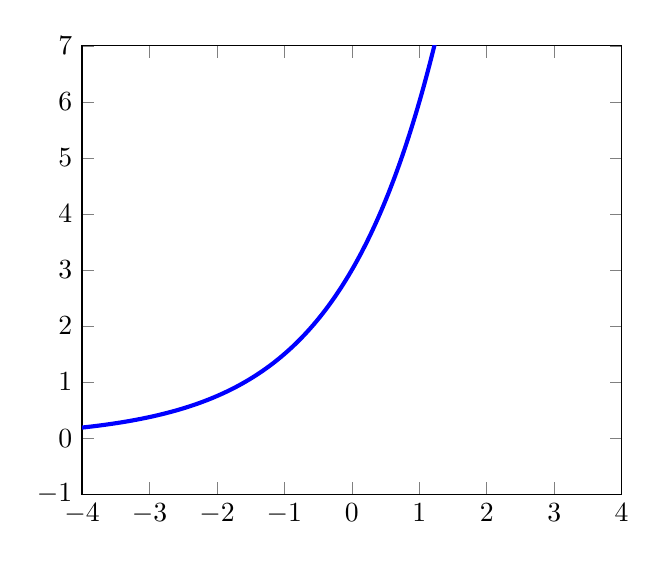
\begin{tikzpicture}
    \begin{axis}[
      xmin=-4,
      xmax=4,
      ymin=-1,
      ymax=7,
      xtick={-6,-5,...,6},
      ytick={-6,-5,...,7}
    ]
    \addplot[line width=1.5pt, blue, smooth, samples=100, restrict y to domain=-2:8] {3*2^(x)};
    \end{axis}
  \end{tikzpicture}
\end{example}

\vspace*{-0.3\textheight}

\newpage

\begin{definition}[The Natural Number $e$]
The natrual number, denoted by $e$, the number that 
${\left (1+\dfrac{1}{n} \right )}^n$ approaches to as $n$ increases without bound. Approximately, $e\approx 2.718282$.
\end{definition}



\begin{example}
  Calculate $e^{3.14}$. Round to five decimal places.
\end{example}

\vspace*{-0.3\textheight}

\begin{note}[Compound Interest]
Let $P$ be the initial amount of the account, known as the principal, $r$ the annual interest rate, and $t$ is the number of years. The balance $A$ after $t$ years is

\begin{itemize}
  \item $A(t)=P{\left (1+\dfrac{r}{n} \right )}^{nt}$ if the interest is compounded $n$ times per year.
  \item $A(t)=Pe^{rt}$ if the interest is compounded continuously ($n\to \infty$).
\end{itemize}
\end{note}
\begin{example}
  We invest $\$3,000$ in an investment account paying $3\%$ interest compounded quarterly, how much will the account be worth in $10$ years?
\end{example}



\begin{example}
  A person invested $\$1,000$ in an account earning $10\%$ per year compounded continuously. How much was in the account at the end of two and a half year?
\end{example}

\newpage

\begin{example}
  A 529 Plan is a college-savings plan that allows relatives to invest money to pay for a child's future college tuition; the account grows tax-free. Lily wants to set up a 529 account for her new granddaughter and wants the account to grow to $\$40,000$ over $18$ years. She believes the account will earn $6\%$ compounded semi-annually (twice a year). To the nearest dollar, how much will Lily need to invest in the account now?
\end{example}

\begin{example}
  $Radon-222$ decays at a continuous rate of $17.3\%$ per day. How much will $100 mg$ of $Radon-222$ decay to in $3$ days?
\end{example}

\newpage
\section*{Exercises}

\begin{exercise}
  A vehicle depriciates according to the formula: $v=27500\left(3.42\right)^{-.04x}$ where $x$ is the age of the car in years. Find the value of the car when it is 14-years old.
\end{exercise}

\begin{exercise}
  Sketch the graph of the function $f(x)=-2\cdot 3^{x-2}+2$.
\end{exercise}

\begin{exercise}
  Find an exponential function $f(x)=ab^x$ that passes through the points $(-2,-6)$ and $(2,-1)$.
\end{exercise}

\newpage

\begin{exercise}
  Find an exponential function $f(x)=ab^x$ graphed in the following figure.\\
  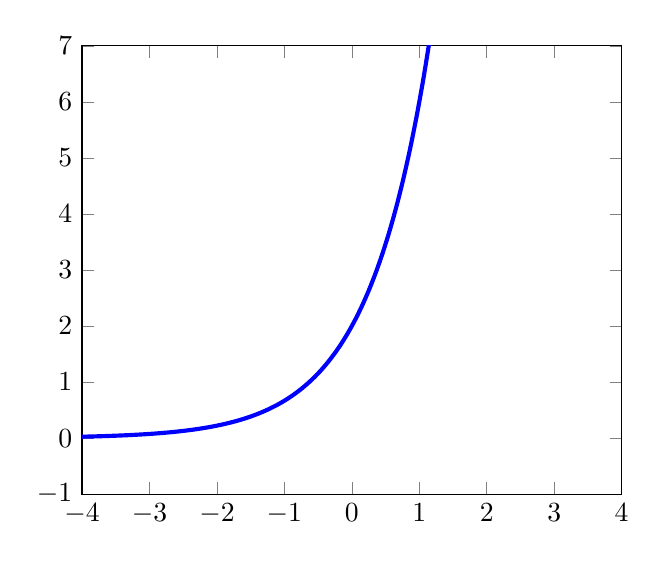
\begin{tikzpicture}
    \begin{axis}[
      xmin=-4,
      xmax=4,
      ymin=-1,
      ymax=7,
      xtick={-6,-5,...,6},
      ytick={-6,-5,...,7}
    ]
    \addplot[line width=1.5pt, blue, smooth, samples=100, restrict y to domain=-2:8] {2*3^(x)};
    \end{axis}
  \end{tikzpicture}
\end{exercise}
\vspace*{-0.25\textheight}

\begin{exercise}
  A wolf population is growing exponentially. In 2011, $129$ wolves were counted. By 2013, the population had reached $236$ wolves. What two points can be used to derive an exponential equation modeling this situation? Write the equation representing the population $N$ of wolves over time $t$.
\end{exercise}

\begin{exercise}
  A scientist begins with $100$ milligrams of a radioactive substance that decays exponentially. After $35$ hours, $50$ mg of the substance remains. How many milligrams will remain after $54$ hours?
\end{exercise}

\newpage

\begin{exercise}
  Consider the function $f(x)=-\dfrac{1}{2e^{-x}+1}$. Find $f(0)$, $f(\sqrt{2})$ and $f(-1)$.
\end{exercise}

\begin{exercise}
  An account is opened with an initial deposit of $\$6,500$ and earns $3.6\%$ interest.
  
  \begin{enumerate}
    \item What will the account be worth in $20$ years if the interest is compounded monthly. 
    \item What will the account be worth in $20$ years if the interest is compounded continuously. 
  \end{enumerate}
\end{exercise}

\newpage
\section{Logarithmic Functions}
\begin{definition}
  Let $y=b^x$ be an exponential function, where $b>0$ and $b\ne 1$. Its inverse function is called the \textbf{logarithmic function with base $b$}, denoted as $\log_b$.
\end{definition}

From the definition of inverse function, for any $x>0$, $\log_bx$, read as the logarithm with base $b$ of $x$, is the unique number such that 
\[b^{\log_bx}=x.\] 
In terms of equations,
\[y=\log_bx\quad \text{is equivalent to}\quad x=b^y.\]

\begin{example}
  Write the following logarithmic equality in exponential form.\\
\begin{enumerate*}
  \item $\log_6(\sqrt{6})=\dfrac{1}{2}$
  \item $\log_3(9)=2$
  \item $\log_2(x)=3$
  \item $\log_x(5)=\dfrac{1}{3}$\hfill\null
\end{enumerate*}
\end{example}

\begin{example}
  Use the exponential form to evaluate the logarithm.\\
  \begin{enumerate*}
    \item $\log_24$
    \item $\log_2\sqrt{2}$
    \item $\log_93$\hfill\null
  \end{enumerate*}
\end{example}

\newpage

\begin{definition}
  A \textbf{common logarithm} is a logarithm with base $10$. We write $\log_{10}(x)$ simply as $\log(x)$.
  
  A \textbf{natural logarithm} is a logarithm with base $e$, the natrual number. We write $\log_{e}(x)$ simply as $\ln(x)$.
\end{definition}

\begin{example}
  Evaluate the logarithm without using a calculator.\\
  \begin{enumerate*}
    \item $\log(1000)$
    \item $\ln(e^2)$\hfill\null
  \end{enumerate*}
\end{example}
\vspace*{-0.1\textheight}

\begin{example}
  Evaluate the logarithm using a calculator.\\
  \begin{enumerate*}
    \item $\log 2$
    \item $\ln 2$\hfill\null
  \end{enumerate*}
\end{example}

\vspace*{-0.1\textheight}

The domain of $y=\log_bx$ is $(0,\infty)$, and the range  is $(-\infty, \infty)$. The function $\log_b$ has an $x$-intercept $(1, 0)$ and a vertical asymptote $x=0$.

If $b>1$, then $y=\log_bx$ is increasing. If $0<b<1$, then $y=\log_bx$ is decreasing.

\begin{example}
  Find the domain of the function.\\
  \begin{enumerate*}
    \item $f(x)=\log_2(x+3)$
    \item $f(x)=\log_3(3-2x)$
    \item $f(x)=\ln(4-x^2)$
    \item $f(x)=\log\left(\dfrac{x+1}{x-2}\right)$\hfill\null
  \end{enumerate*}
\end{example}

\newpage

\begin{example}
  Find an equation for the function $y=\log_bx$ whose graph is shown below.\\
  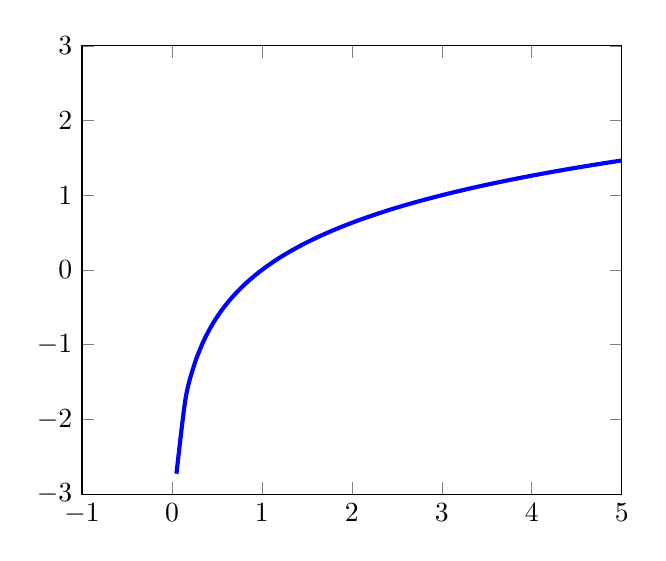
\begin{tikzpicture}
    \begin{axis}[
      xmin=-1,
      xmax=5,
      ymin=-3,
      ymax=3,
      xtick={-6,-5,...,6},
      ytick={-6,-5,...,7}
    ]
    \addplot[line width=1.5pt, blue, smooth, samples=100, restrict y to domain=-4:4] {ln(x)/ln(3)};
    \end{axis}
  \end{tikzpicture}
\end{example}

\vspace*{-0.1\textheight}


\begin{example}
  Find an equation for the function $y=\log_b(x-a)$ whose graph is shown below.\\
  \begin{tikzpicture}
    \begin{axis}[
      xmin=-1,
      xmax=5,
      ymin=-3,
      ymax=3,
      xtick={-6,-5,...,6},
      ytick={-6,-5,...,7}
    ]
    \addplot[line width=1.5pt, blue, smooth, samples=100, restrict y to domain=-4:4] {ln(x-1)/ln(2)};
    \end{axis}
  \end{tikzpicture}
\end{example}

\vspace*{-0.1\textheight}

\begin{example}
  Find the vertical asymptote of $f(x)=-2\log_3(x+4)+5$
\end{example}

\newpage

\section*{Exercises}
\begin{exercise}
  Write the following logarithmic equality in exponential form.\\
\begin{enumerate*}
  \item $\log_42=x$
  \item $\log_3(x)=2$
  \item $\log_x(2)=\dfrac{1}{2}$\hfill\null
\end{enumerate*}
\end{exercise}

\begin{exercise}
  Evaluate the logarithm using a calculator.\\
  \begin{enumerate*}
    \item $\log 3$
    \item $\ln 5$
    \item $\dfrac{\log 5}{\ln 3}$
    \hfill\null
  \end{enumerate*}
\end{exercise}
\vspace*{-0.05\textheight}

\begin{exercise}
  Find the domain of the function.\\
  \begin{enumerate*}
    \item $f(x)=\log_2(2x-1)$
    \item $f(x)=\ln(9-4x^2)$
    \item $f(x)=\log\left(\dfrac{1-x}{x-2}\right)$\hfill\null
  \end{enumerate*}
\end{exercise}
\vspace*{\stretch{1.5}}
\begin{exercise}
  Find an equation for the function $y=-\log_bx$ whose graph is shown below.\\
  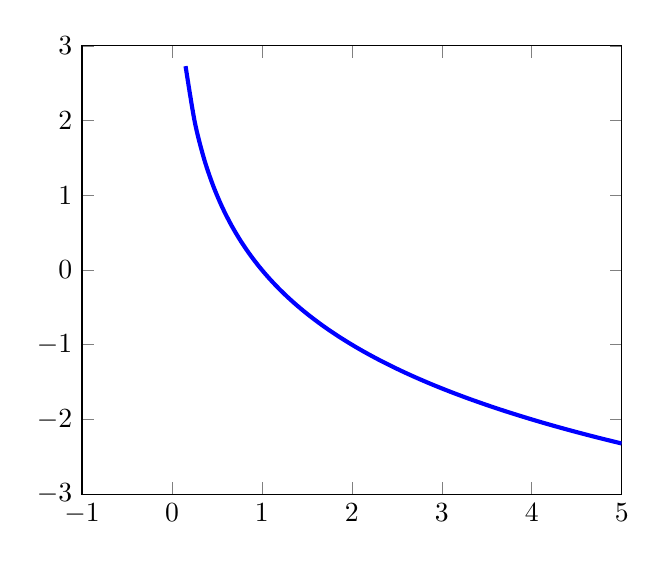
\begin{tikzpicture}
    \begin{axis}[
      xmin=-1,
      xmax=5,
      ymin=-3,
      ymax=3,
      xtick={-6,-5,...,6},
      ytick={-6,-5,...,7}
    ]
    \addplot[line width=1.5pt, blue, smooth, samples=100, restrict y to domain=-4:4] {-ln(x)/ln(2)};
    \end{axis}
  \end{tikzpicture}
\end{exercise}
\vspace*{-0.1\textheight}

\begin{exercise}
  Find the vertical asymptote of $f(x)=-3\log_2(2x-1)+1$
\end{exercise}

\newpage
\section{Properties of Logarithms}

\begin{proposition}[Basic Properties of Logarithms]
 Assume that $b>0$ and $b\neq 1$, and $x>0$. Then

\begin{enumerate}
\item
  $b^{\log_bx}=x$.
\item
  $\log_b(b^x)=x$.
\item
  $\log_bb=1$ and $\log_b1=0$.
\end{enumerate}
\end{proposition}

\begin{example}
Evaluate the logarithm.\\
  \begin{enumerate*}
  \item
    $\log_82$
  \item
    $10^{\log(\frac{1}{2})}$
  \item
    $\log_3(e^0)$\hfill\null
  \end{enumerate*}
\end{example}

\begin{proposition}[Basic Properties of Logarithms]
  Assume $M>0$, $N>0$, $b>0$ and $b\neq 1$. Then 

  \begin{enumerate}
  \item
    (The product rule) $\log_b(MN)=\log_bM+\log_bN$
  \item
    (The quotient rule) $\log_b(\frac MN)=\log_bM-\log_bN$.
  \item
    (The power rule) $\log_b(M^p)=p\log_bM$, where $p$ is any real
    number.
  \item
    (The change-of-base property) $\log_bM=\dfrac{\log_aM}{\log_ab}$,
    where $a>0$ and $a\neq 1$.
     In particular, \[
     \log_bM=\dfrac{\log M}{\log b} \quad\text{and}\quad \log_bM=\dfrac{\ln M}{\ln b}.
     \]
  \end{enumerate}
 \end{proposition}

 \begin{example}
  Expand the logarithmic expression.\\
  \begin{enumerate*}
   \item $\log_3(30x(3x+4))$
   \item $\log\left(\dfrac{2x^2+6x}{3x+9} \right)$
   \item $\log_2(\sqrt{x^2+1})$
   \item $\ln\left (\dfrac{x^4(y-1)}{x^2+1}\right)$
   \hfill\null
  \end{enumerate*}
 \end{example}

 \newpage

 \begin{example}
  Evaluate the logarithm using calculator.\\
  \begin{enumerate*}
    \item $\log_25$
    \item $\log_35-\log 53$
    \item $\dfrac{\log_23}{\log_32}$\hfill\null
  \end{enumerate*}
 \end{example}
 
\vspace*{-0.2\textheight}

\begin{example}
  Expand the logarithmic expression
  \[\ln \left (\dfrac{\sqrt{(x-1){(2x+1)}^2}}{(x^2-9)}\right ).\]
\end{example}

\begin{example}
  Condense the logarithmic expression.\\
  \begin{enumerate*}
    \item $\log_2(x^2)+\dfrac{1}{2}\log_2(x-1)-3\log_2({(x+3)}^2)$
    \item $3\ln(x)-\dfrac{1}{2}\ln(x+1)-2\ln(\sqrt{x^2+3})$ \hfill\null
  \end{enumerate*}
\end{example}

\newpage

\section*{Exercises}

\begin{exercise}
    Expand the logarithmic expression.\\
    \begin{enumerate*}
     \item $\log_6\left(\dfrac{64x^3(4x+1)}{(2x-1)} \right)$.
     \item $\ln\left(\dfrac{\sqrt{(x-1)}(2x+1)^2}{(x^2-9)}\right)$
     \hfill\null
    \end{enumerate*}
\end{exercise}

\begin{exercise}
  Condense the logarithmic expressions.\\
  \begin{enumerate*}
    \item $2\log x-4\log(x+5)+\dfrac{1}{3}\log(3x+5)$
    \item $4(3\log(x)+\log(x+5)-\log(2x+3))$
  \end{enumerate*}
\end{exercise}

\begin{exercise}
  Evaluate the logarithm using a calculator.\\
  \begin{enumerate*}
    \item $\log_5{23}$
    \item $\log_49-\log5$
    \item $\dfrac{\ln10}{\log_5{10}}$\hfill\null
  \end{enumerate*}
\end{exercise}

\newpage
\section{Exponential and Logarithmic Equations}

\begin{howto}[Exponential equation]
 Isolate an exponential expression first and then take logarithm with the same base, or any base of both sides. After that, solve the resulting equation.
\end{howto}

\begin{example}
  Solve\\ 
  \begin{enumerate*}
    \item $3^{x+1}=4$
    \item $2^{x-1}=2^{2x-4}$
    \item $8^{x+2}={16}^{x+1}$
    \item $5^{x+2}=4^x$
  \end{enumerate*}  
\end{example}

\begin{example}
  Solve\\ 
  \begin{enumerate*}
    \item $100=20e^{2t}$
    \item $4e^{2x}+5=12$
    \item $e^{2x}-e^x=56$
  \end{enumerate*}  
\end{example}

\newpage

\begin{howto}[Logarithmic equation]
  Isolate a logarithmic expression first and then apply the exponential function with the same base. After that, solve the resulting equation.
\end{howto}

\begin{example}
  Solve\\
\begin{enumerate*}
  \item $2\ln x+3=7$
  \item $\ln(x^2)=\ln(2x+3)$
  \item $-\dfrac{1}{2}\log (x+1)-3=0$
  \item $\ln (x)-\ln (x+3)=\ln 6$
\end{enumerate*}
\end{example}


\begin{example}
  The population of a small town is modeled by the equation $P=1650e^{0.5t}$ where $t$ is measured in years. In approximately how many years will the town's population reach $20,000$?
\end{example}

\newpage

\begin{example}
  The magnitude $M$ of an earthquake is represented by the equation $M=\dfrac{2}{3}\log\left( \dfrac{E}{E_0} \right)$ where $E$ is the amount of energy released by the earthquake in joules, and $E_0=10^{4.8}$ is the assigned minimal measure released by an earthquake. To the nearest hundredth, if the magnitude of an earthquake is 7.8, how much energy was released?
\end{example}

\begin{example}
  An account with an initial deposit of $\$6,500$ earns $7.25\%$ annual interest, compounded monthly. After how many years, the balance will be doubled.
\end{example}


\newpage

\section*{Exercises}

\begin{exercise}
  Solve\\ 
  \begin{enumerate*}
    \item $3^{1-x}=5$
    \item $3^{x-2}=4^{2x}$
    \item $5=10^{3t-2}$
    \item $e^{2x}-2e^x=15$
  \end{enumerate*}  
\end{exercise}

\begin{exercise}
  Solve\\
\begin{enumerate*}
  \item $2\log x-3=-1$
  \item $\ln(2x^2)=\ln(5x+3)$
  \item $\dfrac{1}{2}\log_2(3x-1)=2$
  \item $\ln(x-1)-\ln(x+1)=1$
\end{enumerate*}
\end{exercise}


\newpage
\section{Exponential and Logarithmic Models}

\begin{howto}[Exponential Growth or Decay]
  The function
  \[A(t)=A_0e^{kt}\]
is frequently used to model exponential growth (when $k>0$) or decay (when $k<0$), where $A_0$ is the initial quantity.
\end{howto}

\begin{example}
  A population of bacteria doubles every hour. A culture started with 10 bacteria.
  \begin{enumerate}
    \item After 6 hours how many bacteria will there be?
    \item After how many hours will the population be tripled?  
  \end{enumerate}
\end{example}


\begin{example}
  The half-life of carbon-14 is $5,730$ years. A bone fragment is found that contains  20\% of its original carbon-14. To the nearest year, how old is the bone?
\end{example}

\newpage

\begin{example}
  Sam goes to the doctor and the doctor gives him $15$ milligrams of radioactive dye. After $15$ minutes, $9$ milligrams of dye remain in Sam body. To leave the doctor's office, Sam must pass through a radiation detector that will sound the alarm if more than 2 milligrams of the dye are in his body. How long Sam's visit to the doctor take, assuming he was given the dye as soon as he arrived?
\end{example}

\begin{howto}[Newton's Law of Cooling]
  The temperature of an object, $T$, in surrounding air with constant temperature $T_s$, will behave according to the formula
  $$T(t)=Ae^{kt}+T_s,$$
where $t$ is time, $A$ is the difference between the initial temperature of the object and the surroundings, $k$ is a constant, the continuous rate of cooling of the object.
\end{howto}

\begin{example}
  A cheesecake is taken out of the oven with an ideal internal temperature of $165\unit{\degree F}$, and is placed into a $35\unit{\degree F}$ refrigerator. After $10$ minutes, the cheesecake has cooled to $150\unit{\degree F}$. If we must wait until the cheesecake has cooled to $70\unit{\degree F}$ before we eat it, how long will we have to wait?
\end{example}

\newpage
\begin{howto}[Logistic Growth Model]
  The logistic growth model is approximately exponential at first, but it has a reduced rate of growth as the output approaches the model's upper bound, called the carrying capacity. The logistic growth of a population over time $t$ is represented by the model
  \[P(t)=\dfrac{c}{1+ae^{-bt}},\]
  where $a$, $b$ and $c$ are positive constants, and $b$ is the growth rate, $c$ is the capacity.
\end{howto}

\begin{example}
  The equation  $N(t)=\dfrac{500}{1+49e^{-0.7t}}$ models the number of people in a small town who have heard a rumor after $t$ days.
  \begin{enumerate}
    \item What's the population of the small town?
    \item How many people started the rumor?
    \item To the nearest whole number, how many people will have heard the rumor after $3$ days?
  \end{enumerate}
\end{example}

\newpage

\section*{Exercises}

\begin{exercise}
  A bacteria culture initially contains $3000$ bacteria and doubles every half hour. Find the size of the bacteria population after $80$ minutes.
\end{exercise}

\begin{exercise}
  The half-life of tritium-3 is 12.25 years. How long would it take the sample to decay to 20\% of its original amount?
\end{exercise}

\begin{exercise}
  A doctor prescribes $125$ milligrams of a therapeutic drug that decays by about $30\%$ each hour.
  \begin{enumerate}
    \item To the nearest hour, what is the half-life of the drug?
    \item How long would it take the drug to decay to $30\%$ of its original amount.
  \end{enumerate}
\end{exercise}

\newpage

\begin{exercise}
  A cup of coffee at $185\unit{\degree F}$ is placed into a $60\unit{\degree F}$ room. One hour later, the temperature of coffee has dropped to $120\unit{\degree F}$. How long will it take for the temperature to drop to $80\unit{\degree F}$?
\end{exercise}

\begin{exercise}
  The population of a fish farm in $t$ years is modeled by the equation $P(t)=\dfrac{1000}{1+9e^{-0.6t}}$.
\begin{enumerate}
  \item What is the initial population of fish?
  \item To the nearest tenth, what is the doubling time for the fish population?
\end{enumerate}
\end{exercise}




